\documentclass[11pt, oneside]{article}   	% use "amsart" instead of "article" for AMSLaTeX format
\usepackage{geometry}                		% See geometry.pdf to learn the layout options. There are lots.
\geometry{letterpaper}                   		% ... or a4paper or a5paper or ... 
%\geometry{landscape}                		% Activate for rotated page geometry
%\usepackage[parfill]{parskip}    		% Activate to begin paragraphs with an empty line rather than an indent
\usepackage{graphicx}				% Use pdf, png, jpg, or eps§ with pdflatex; use eps in DVI mode
								% TeX will automatically convert eps --> pdf in pdflatex		
\usepackage{amssymb}

%SetFonts

%SetFonts
\setlength{\parindent}{0pt}

\title{Summary of Centrality Metrics' Performance Comparisons on Stock Market Datasets Paper}
\author{Jody Shu}
%\date{}							% Activate to display a given date or no date

\begin{document}
\begin{Large}
\maketitle
%\section{}
%\subsection{}
The authors applied centrality metrics methods which are betweenness, closeness, eigenvector, PageRank and weighted degree measurements to top 300 stocks.  Graph centrality measurements using degree and PageRank factors can provide information with importance ranking in the stock market to offer stakeholders a general idea on their future investments.  In the article, the authors used each share as a 'node' and a realtion between one stock and another is considered an 'edge'.  

In the concept of centrality metrics, a stock network is a labelled undirected weighted graph G = (V, E, w), in which V presents the set of vertices, E is the set of edges and w is the weight function.  There are five metrics adopted in this paper.



In this study, the eigenvector centrality concept is adopted in undirected graphs as a ranking measure to analyse the importance of stocks; it measures the extent to which a stock interacts with other shares in the stock market. Let A show an $(n\times n)$similarity matrix, $\lambda$ be the largest eigenvalue of A and x the corresponding eigenvector, the eigenvector centrality $x_i$ of node i is defined as the $i^{th}$ entry in the normalized eigenvector belonging to the largest eigenvalue of A, N(i) are the node i’s neighboring nodes, consider a particular node i with its adjacent nodes N(i), then
$x_i=\sum_{j\in N(i)} A_{ij}x{j}$\\

As for the PageRank algorithm, the weighted degree $x_i$ of a node i is the sum of weight values that from all nodes connect to it, the weight is defined as:

$x_i=\sum_{j\in V} w_{ij}$

In conclusion, after they conducted the study, the following is a table of a similarity rates from the 5 methods they used.

\begin{figure}[htbp] %  figure placement: here, top, bottom, or page
   \centering
   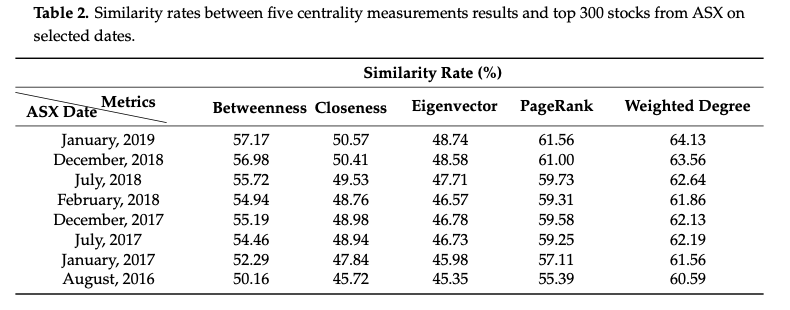
\includegraphics[width=6in]{comparison_of_similarity} 
  % \caption{}
   %\label{fig:example}
\end{figure}

There are some factors that the authors didn't take into account for this study which resulted that the outcomes are not the same as the ASX (Australian Securities Exchange) entirely, and one of the reasons for that was because they didn't factor the stock's market cash flow.  And the future work for them will include looking at cycles and symmetry in the stock market.




\end{Large}
\end{document}  